\documentclass[../ei103948-project-documentation.tex]{subfiles}
\begin{document}

\section{Organización}
\subsection{Proyecto}

El proyecto está organizado según una jerarquía muy sencilla, básicamente se divide en tres grandes grupos con cada uno teniendo una ruta concreta, los cuales detallaremos a continuación.

    \begin{itemize}
        \item \textbf{Tests}: \texttt{src/test/java}
        \item \textbf{Backend}: \texttt{src/mains/java}
        \item \textbf{Frontend}: \texttt{src/main/webapp}
    \end{itemize}

La construcción del proyecto es también es sencilla, puedes utilizar las herramientas proporcionadas por tu propio editor o ejecutar la acción de clonado de \textbf{Git} con la opción \texttt{{-}{-}recurse-submodules}. Luego basta con ejecutar un \textbf{Maven} \textit{goal}, por defecto el proyecto dispone de muchos en uso normal solo se utilizaran tres básicamente, lo cuales detallaremos a continuación:

\begin{itemize}
    \item \textbf{Limpiar entorno}: \texttt{mvn clean}
    \item \textbf{Ejecutar}: \texttt{mvn spring-boot:run}
    \item \textbf{Ejecutar tests}:  \texttt{mvn -P-webapp test}
\end{itemize}

Si se han realizado cambios y el proyecto se va ejecutar desde un editor, ya sea para una ejecución normal o para tests, es recomendable inicializarlo al menos una vez mediante el \textit{goal}. Luego, si se quiere, se pueden repetir ejecuciones sin ningún problema.\\

El servidor, por defecto, se encontrará en: http://localhost:8080/.

\subsection{Interfaz de Programación de Aplicaciones -- API}
El término \textit{API}\cite{api-xataka} es una abreviatura de \textit{Application Programming Interfaces}, que en español significa interfaz de programación de aplicaciones. Se trata de un conjunto de definiciones y protocolos que se utiliza para desarrollar e integrar el software de las aplicaciones, permitiendo la comunicación entre dos aplicaciones de software a través de un conjunto de reglas.\\

Así pues, podemos hablar de una \textit{API} como una especificación formal que establece cómo un módulo de un software se comunica o interactúa con otro para cumplir una o muchas funciones. Todo dependiendo de las aplicaciones que las vayan a utilizar, y de los permisos que les dé el propietario de la \textit{API} a los desarrolladores de terceros.\\

\begin{figure}[H]
    \begin{center}
    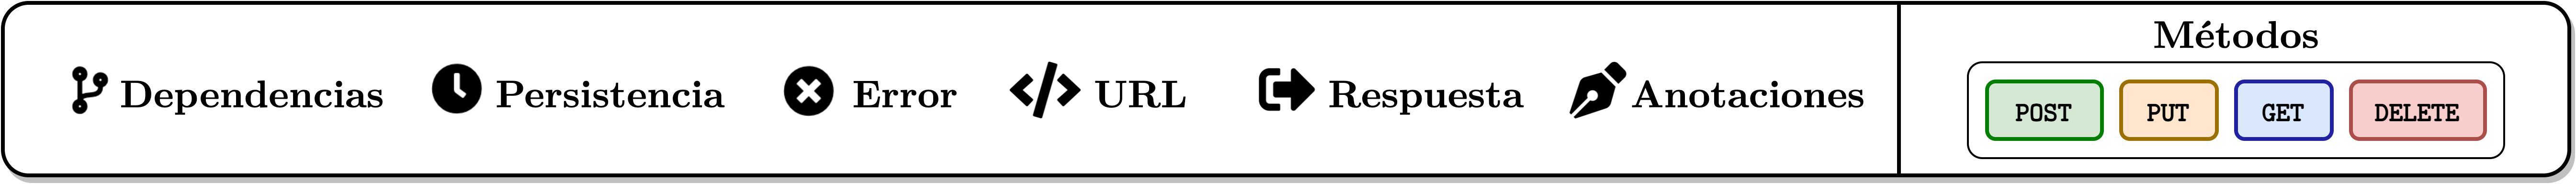
\includegraphics[scale=0.083]{images/BannerAPI.png}
    \end{center}
\end{figure}

%[\faIcon{sign-out-alt}] = Respuesta
%[\faIcon{pen-nib}] = Anotación
%[\faIcon{code}] = Código o URL

        \subsubsection{Tipos de datos}
            \paragraph{Básicos}
                \paragraph*{\texttt{Account}}
                    \begin{itemize}
                        \item [\faIcon{sign-out-alt}] : \texttt{\{mail: string, transient: boolean\}}
                    \end{itemize}
                \paragraph*{\texttt{Location}}
                    \begin{itemize}
                        \item [\faIcon{sign-out-alt}] : \texttt{\{coords: string, name: string, alias: string\}}
                    \end{itemize}
                \paragraph*{\texttt{Service}}
                    \begin{itemize}
                        \item [\faIcon{sign-out-alt}] : \texttt{\{type: string, name: string, description: string\}}
                        \item [\faIcon{pen-nib}] \quad \faIcon{arrow-down} :
                            \begin{itemize}
                                \item \texttt{type}: mirar sección de \hyperref[sec:respuestasservicios]{\underline{respuestas de servicios}}.
                            \end{itemize}
                    \end{itemize}

                    
        \subsubsection{Respuestas de servicios}
        \label{sec:respuestasservicios}
        \paragraph{\texttt{WEATHER}}
                \begin{itemize}
                    \item [\faIcon{sign-out-alt}] : \texttt{\{icon: URL, description: string, temp: number, url\}}
                    \item [\faIcon{pen-nib}] \quad \faIcon{arrow-down} :
                        \begin{itemize}
                            \item  \texttt{temp}: en celsius.
                            \item  \texttt{rain}: probabilidad (de 0 a 1).
                            \item  \texttt{wind}: en m/s.
                        \end{itemize}
                    \end{itemize}


            \paragraph{\texttt{EVENTS}}
            \begin{itemize}
                \item [\faIcon{sign-out-alt}] : \texttt{[\{title: string, date: string, location: string, author: string, url: URL, image: URL, price: number\}, ...]}
                \item [\faIcon{pen-nib}] \quad \faIcon{arrow-down} :
                    \begin{itemize} 
                        \item  \texttt{price}: en euros y en caso de no estar disponible contendrá \texttt{false}.
                        \item  \texttt{date}: en formato \href{https://www.iso.org/obp/ui/#iso:std:iso:8601:-1:ed-1:v1:en}{\underline{ISO 8601} \faIcon{book}}.
                    \end{itemize}
                \end{itemize}

            \blfootnote{
                \begin{figure}[H]
                    \begin{center}
                    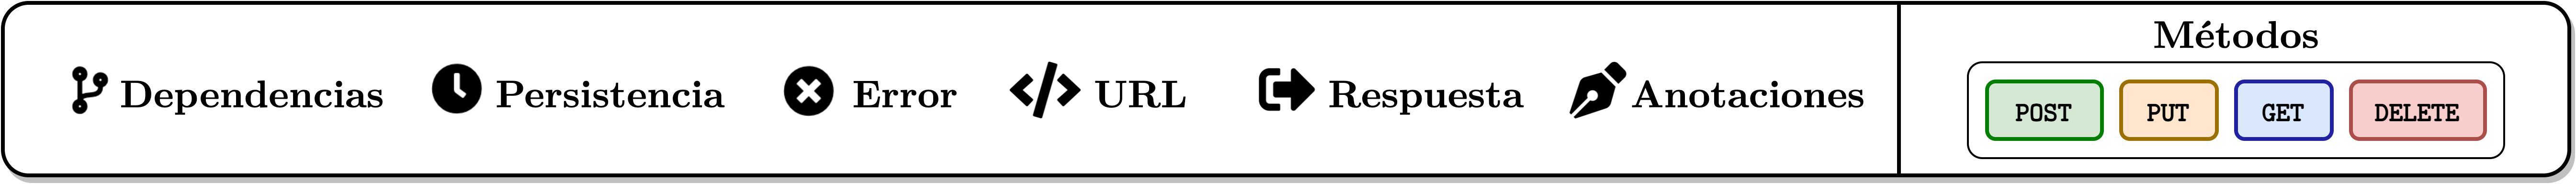
\includegraphics[scale=0.083]{images/BannerAPI.png}
                    \end{center}
                \end{figure}
            }

            \paragraph{\texttt{NEWS}}
            \begin{itemize}
                \item [\faIcon{sign-out-alt}] : \texttt{[\{title: string, description: string, author: string, url: URL, image: URL\}, ...]}
                \item [\faIcon{pen-nib}] \quad \faIcon{arrow-down} :
                    \begin{itemize} 
                        \item  \texttt{image}: en caso de no estar disponible contendrá \texttt{false}.
                    \end{itemize}
                \end{itemize}





        \subsubsection{Peticiones}
        Salvo que se especifique lo contrario se asume lo siguiente para todas las peticiones:
                \begin{itemize}
                    \item \textbf{Respuesta}: ninguna.
                    \item \textbf{Error}: en caso de no tener \textit{session} $\rightarrow$ \texttt{401 Unauthorized}.
                    \item \textbf{Dependencias}: ninguna.
                \end{itemize}
            \paragraph{Cuentas}

                    \begin{itemize}
                        \item \textbf{Gestión}
                        \begin{itemize}
                            \setlength\itemsep{0.5cm}
                            \item \underline{\textbf{Registrar}}
                            \begin{itemize}
                                \item [\faIcon{cog}] : \makebox{\posttext}
                                \item [\faIcon{code}] : \texttt{/account?mail=\{mail\}\&password=\{password\}}
                                \item [\faIcon{times-circle}] : en caso de cuenta existente $\rightarrow$ \texttt{409 Conflict}.
                                \item [\faIcon{clock}] : modificada.
                                \item [\faIcon{pen-nib}] \quad \faIcon{arrow-down} :
                                    \begin{itemize}
                                        \item Sesión no necesaria.
                                        \item Implicitamente inicia sesión.
                                    \end{itemize}
                            \end{itemize}
    
                            \item \underline{\textbf{Actualizar}}
                                \begin{itemize}
                                    \item [\faIcon{cog}] : \makebox{\puttext}
                                    \item [\faIcon{code}] : \texttt{/account?password=\{password\}}
                                    \item [\faIcon{clock}] : modificada.
                                \end{itemize}

                                {}\blfootnote{
                                    \begin{figure}[H]
                                        \begin{center}
                                        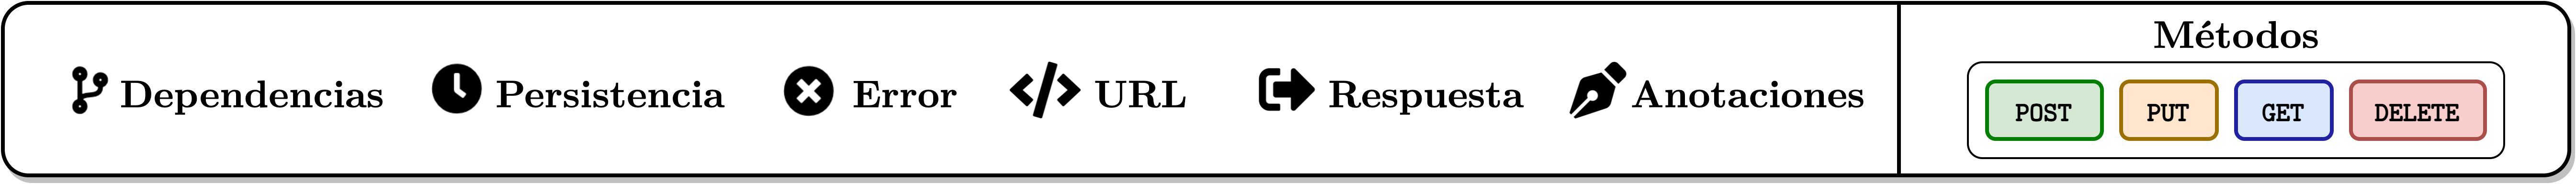
\includegraphics[scale=0.083]{images/BannerAPI.png}
                                        \end{center}
                                    \end{figure}
                                }
    
                            \item \underline{\textbf{Dar de baja}}
                            \begin{itemize}
                                \item [\faIcon{cog}] : \makebox{\deletetext}
                                \item [\faIcon{code}] : \texttt{/account}
                                \item [\faIcon{clock}] : modificada.
                            \end{itemize}
                        \end{itemize}
                        

                        \item \textbf{Sesión}
                        \begin{itemize}
                            \setlength\itemsep{0.5cm}
                                \item \underline{\textbf{Estado}}
                                \begin{itemize}
                                    \item [\faIcon{cog}] : \makebox{\gettext}
                                    \item [\faIcon{code}] : \texttt{/session}
                                    \item [\faIcon{sign-out-alt}] : \texttt{Account}.
                                    \item [\faIcon{times-circle}] : en caso de datos incorrectos $\rightarrow$ \texttt{401 Unauthorized}.
                                    \item [\faIcon{pen-nib}] \quad \faIcon{arrow-down} :
                                        \begin{itemize}
                                            \item Sesión no necesaria.
                                        \end{itemize}
                                \end{itemize}

                                \item \underline{\textbf{Iniciar}}
                                \begin{itemize}
                                    \item [\faIcon{cog}] : \makebox{\posttext}
                                    \item [\faIcon{code}] : \texttt{/session?mail=\{mail\}\&password=\{password\}}
                                    \item [\faIcon{times-circle}] : en caso de datos incorrectos $\rightarrow$ \texttt{401 Unauthorized}.
                                    \item [\faIcon{pen-nib}] \quad \faIcon{arrow-down} :
                                        \begin{itemize}
                                            \item Sesión no necesaria.
                                        \end{itemize}
                                \end{itemize}


                                \item \underline{\textbf{Iniciar como invitado}}
                                \begin{itemize}
                                    \item [\faIcon{cog}] : \makebox{\posttext}
                                    \item [\faIcon{code}] : \texttt{/session/guest}
                                    \item [\faIcon{pen-nib}] \quad \faIcon{arrow-down} :
                                        \begin{itemize}
                                            \item Sesión no necesaria.
                                        \end{itemize}
                                \end{itemize}

                                \item \underline{\textbf{Cerrar}}
                                \begin{itemize}
                                    \item [\faIcon{cog}] : \makebox{\deletetext}
                                    \item [\faIcon{code}] : \texttt{/session}
                                \end{itemize}
                            \end{itemize}
                    \end{itemize}

                    {}\blfootnote{
                        \begin{figure}[H]
                            \begin{center}
                            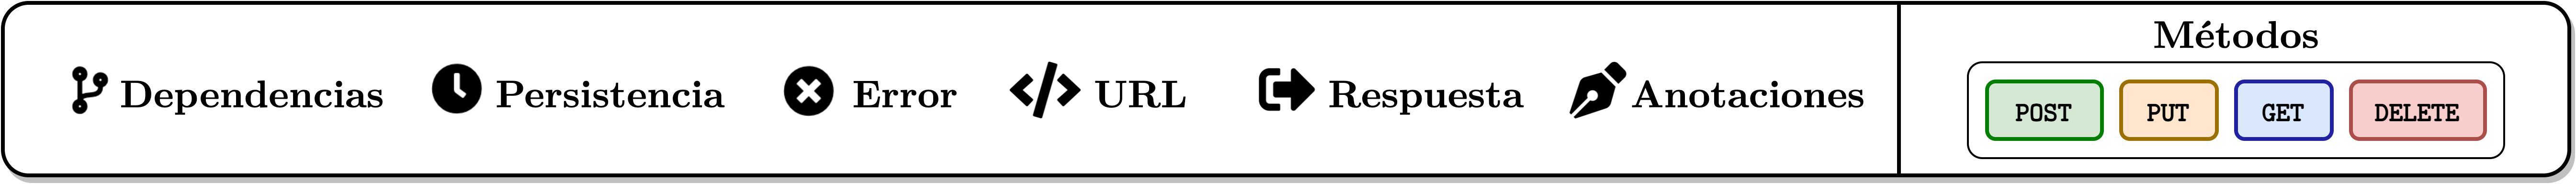
\includegraphics[scale=0.083]{images/BannerAPI.png}
                            \end{center}
                        \end{figure}
                    }


                \paragraph{Ubicaciones}
                \begin{itemize}
                    \setlength\itemsep{0.5cm}
                    \item \textbf{Búsqueda}
                    \begin{itemize}
                            \item [\faIcon{cog}] : \makebox{\gettext}
                            \item [\faIcon{code}] : \texttt{ /query/\{query\}}
                            \item [\faIcon{sign-out-alt}] : \texttt{[Location, ...]}
                            \item [\faIcon{code-branch}] : búsqueda.
                        \end{itemize}
                    

                    \item \textbf{Actuales}
                    \begin{itemize}
                        \setlength\itemsep{0.5cm}
                        \item \underline{\textbf{Obtener}}
                        \begin{itemize}
                            \item [\faIcon{cog}] : \makebox{\gettext}
                                \item [\faIcon{code}] : \texttt{/locations}
                                \item [\faIcon{sign-out-alt}] : \texttt{[Location, ...]}
                                \item [\faIcon{code-branch}] : búsqueda.
                            \end{itemize}
                            
                        \item \underline{\textbf{Añadir}}
                        \begin{itemize}
                            \item [\faIcon{cog}] : \makebox{\posttext}
                                \item [\faIcon{code}] : \texttt{/locations/\{query\}?alias=\{name\}}
                                \item [\faIcon{sign-out-alt}] : \texttt{Location}
                                \item [\faIcon{times-circle}] :  En caso de no encontrar el lugar $\rightarrow$ \texttt{404 Not Found}.
                                \item [\faIcon{code-branch}] : búsqueda.
                                \item [\faIcon{clock}] : modificada.
                                \item [\faIcon{pen-nib}] \quad \faIcon{arrow-down} :
                                    \begin{itemize}
                                        \item \texttt{query}: preferiblemente utilizar coordenadas.
                                        \item \texttt{alias}: si no se ha especificado, se utilizará el topónimo.
                                    \end{itemize}
                            \end{itemize}

                        \item \underline{\textbf{Modificar}}
                        \begin{itemize}
                            \item [\faIcon{cog}] : \makebox{\puttext}
                                \item [\faIcon{code}] : \texttt{/locations/\{coords\}?alias=\{name\}}
                                \item [\faIcon{sign-out-alt}] : \texttt{Location}.
                                \item [\faIcon{clock}] : ninguna.
                            \end{itemize}

                            {}\blfootnote{
                                \begin{figure}[H]
                                    \begin{center}
                                    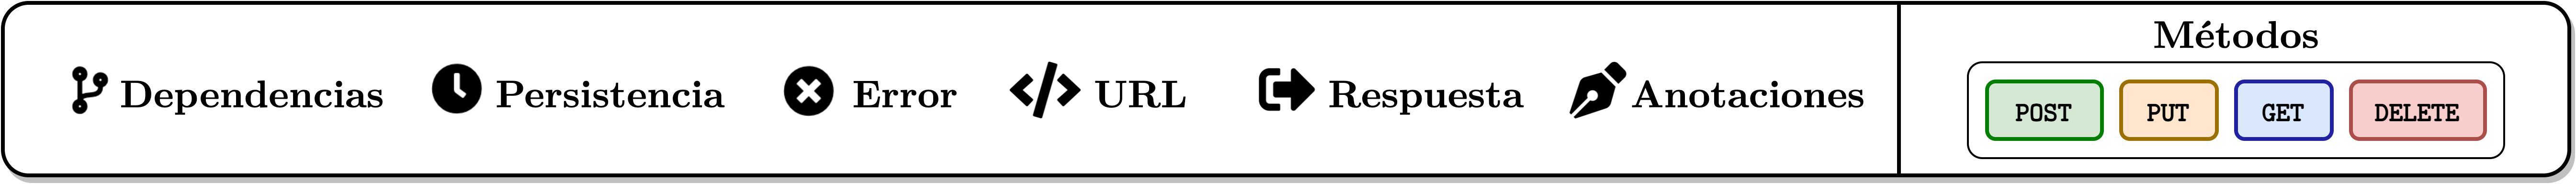
\includegraphics[scale=0.083]{images/BannerAPI.png}
                                    \end{center}
                                \end{figure}
                            }

                        \item \underline{\textbf{Eliminar}}
                        \begin{itemize}
                            \item [\faIcon{cog}] : \makebox{\deletetext{}}
                                \item [\faIcon{code}] : \texttt{/locations/\{coords\}}
                                \item [\faIcon{clock}] : modificada.
                            \end{itemize}

                            \end{itemize}

                    \item \textbf{Históricas}
                            \begin{itemize}
                                \setlength\itemsep{0.5cm}
                                \item \underline{\textbf{Listar}}
                                \begin{itemize}
                                    \item [\faIcon{cog}] : \makebox{\gettext}
                                        \item [\faIcon{code}] : \texttt{/history}
                                        \item [\faIcon{sign-out-alt}] : \texttt{[Place, ...]}
                                    \end{itemize}

                                \item \underline{\textbf{Restaurar}}
                                \begin{itemize}
                                    \item [\faIcon{cog}] : \makebox{\posttext}
                                        \item [\faIcon{code}] : \texttt{/history/\{coords\}}
                                        \item [\faIcon{clock}] : modificada.
                                    \end{itemize}

                                \item \underline{\textbf{Eliminar}}
                                \begin{itemize}
                                    \item [\faIcon{cog}] : \makebox{\deletetext}
                                        \item [\faIcon{code}] : \texttt{/history/\{coords\}}
                                        \item [\faIcon{clock}] : modificada.
                                    \end{itemize}
                            \end{itemize}
                    \end{itemize}

                
                    \paragraph{Servicios}
                    \begin{itemize}
                    \item \textbf{Nivel de cuenta}
                    \begin{itemize}
                        \setlength\itemsep{0.5cm}
                        \item \underline{\textbf{Obtener}}
                        \begin{itemize}
                            \item [\faIcon{cog}] : \makebox{\gettext}
                                \item [\faIcon{code}] : \texttt{/services}
                                \item [\faIcon{sign-out-alt}] : \texttt{[\{service: Service, enabled: boolean\}, ...]}
                            \end{itemize}

                            {}\blfootnote{
                                \begin{figure}[H]
                                    \begin{center}
                                    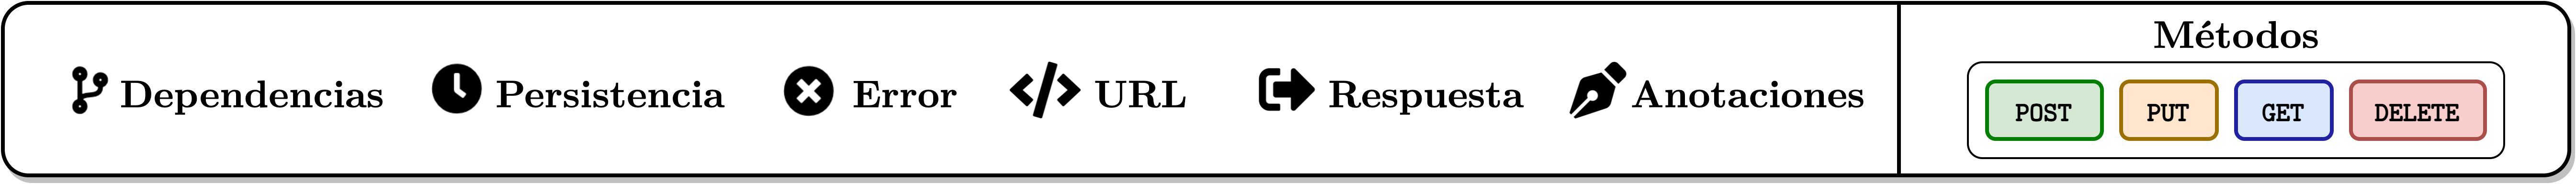
\includegraphics[scale=0.083]{images/BannerAPI.png}
                                    \end{center}
                                \end{figure}
                            }
                            
                        \item \underline{\textbf{Habilitar}}
                        \begin{itemize}
                            \item [\faIcon{cog}] : \makebox{\posttext}
                                \item [\faIcon{code}] : \texttt{/services?type=\{type\}}
                                \item [\faIcon{clock}] : modificada.
                                \item [\faIcon{pen-nib}] \quad \faIcon{arrow-down} :
                                \begin{itemize}
                                    \item \texttt{type}: sí no especificado deshabilita todos los disponibles.
                                \end{itemize}
                            \end{itemize}

                        \item \underline{\textbf{Deshabilitar}}
                        \begin{itemize}
                            \item [\faIcon{cog}] : \makebox{\deletetext}
                                \item [\faIcon{code}] : \texttt{/services?type=\{type\}}
                                \item [\faIcon{clock}] : modificada.
                                \item [\faIcon{pen-nib}] \quad \faIcon{arrow-down} :
                                \begin{itemize}
                                    \item \texttt{type}: sí no especificado deshabilita todos los disponibles.
                                \end{itemize}
                            \end{itemize}

                        \end{itemize}

                        \item \textbf{Nivel de lugar}
                        \begin{itemize}
                            \setlength\itemsep{0.5cm}
                            \item \underline{\textbf{Obtener}}
                            \begin{itemize}
                                \item [\faIcon{cog}] : \makebox{\gettext}
                                    \item [\faIcon{code}] : \texttt{/services/\{query\}}
                                    \item [\faIcon{sign-out-alt}] \texttt{[\{service: Service, enabled: boolean, data: Response\}, ...]}
                                    \item [\faIcon{code-branch}] : búsqueda y servicios.
                                    \item [\faIcon{pen-nib}] \quad \faIcon{arrow-down} :
                                        \begin{itemize}
                                            \item \texttt{query}: preferiblemente utilizar coordenadas.
                                            \item \texttt{data}: en caso de servicio inactivo o error contendrá \texttt{false}.
                                        \end{itemize}
                                \end{itemize}
                                
                            \item \underline{\textbf{Habilitar}}
                            \begin{itemize}
                                \item [\faIcon{cog}] : \makebox{\posttext}
                                    \item [\faIcon{code}] : \texttt{/services/\{coords\}?type=\{type\}}
                                    \item [\faIcon{clock}] : modificada.
                                    \item [\faIcon{pen-nib}] \quad \faIcon{arrow-down} :
                                    \begin{itemize}
                                        \item \texttt{type}: sí no especificado habilita todos los disponibles.
                                    \end{itemize}
                                \end{itemize}

                                {}\blfootnote{
                                    \begin{figure}[H]
                                        \begin{center}
                                        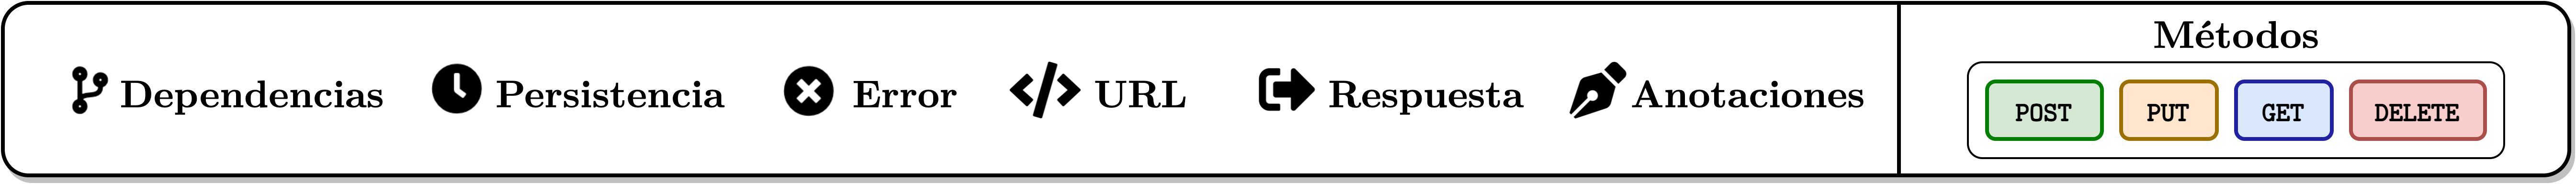
\includegraphics[scale=0.083]{images/BannerAPI.png}
                                        \end{center}
                                    \end{figure}
                                }

                            \item \underline{\textbf{Deshabilitar}}
                            \begin{itemize}
                                \item [\faIcon{cog}] : \makebox{\deletetext}
                                    \item [\faIcon{code}] : \texttt{/services/\{coords\}?type=\{type\}}
                                    \item [\faIcon{clock}] : modificada.
                                    \item [\faIcon{pen-nib}] \quad \faIcon{arrow-down} :
                                    \begin{itemize}
                                        \item \texttt{type}: sí no especificado deshabilita todos los disponibles.
                                    \end{itemize}
                                \end{itemize}

                    \end{itemize}

                    \end{itemize}

   



\end{document}